% Use only LaTeX2e, calling the article.cls class and 12-point type.

\documentclass[12pt]{article}

% Users of the {thebibliography} environment or BibTeX should use the
% scicite.sty package, downloadable from *Science* at
% http://www.sciencemag.org/authors/preparing-manuscripts-using-latex 
% This package should properly format in-text
% reference calls and reference-list numbers.

\usepackage{scicite}

\usepackage{times}

\usepackage{graphicx}

\usepackage{caption}

\PassOptionsToPackage{hyphens}{url}\usepackage{hyperref}

% The preamble here sets up a lot of new/revised commands and
% environments.  It's annoying, but please do *not* try to strip these
% out into a separate .sty file (which could lead to the loss of some
% information when we convert the file to other formats).  Instead, keep
% them in the preamble of your main LaTeX source file.


% The following parameters seem to provide a reasonable page setup.

\topmargin 0.0cm
\oddsidemargin 0.2cm
\textwidth 16cm 
\textheight 21cm
\footskip 1.0cm


%The next command sets up an environment for the abstract to your paper.

\newenvironment{sciabstract}{%
\begin{quote} \bf}
{\end{quote}}



% Include your paper's title here

\title{Modeling Water Buffalo Movement} 


% Place the author information here.  Please hand-code the contact
% information and notecalls; do *not* use \footnote commands.  Let the
% author contact information appear immediately below the author names
% as shown.  We would also prefer that you don't change the type-size
% settings shown here.

\author
{George Khoury and Eric Prologo\\
\\
\normalsize{Department of Computer Science, University of Colorado Boulder,}\\
\normalsize{1600 Pleasant St.
275 UCB
Boulder, CO 80309-0275}\\
}

% Include the date command, but leave its argument blank.

\date{}



%%%%%%%%%%%%%%%%% END OF PREAMBLE %%%%%%%%%%%%%%%%



\begin{document} 

% Double-space the manuscript.

\baselineskip24pt

% Make the title.

\maketitle 



% Place your abstract within the special {sciabstract} environment.

\begin{sciabstract}
As the number of wild Water Buffaloes diminishes, understanding their movement patterns and behavior is becoming increasingly imperative. As a herd animal whose movement relies heavily on its environment, the water buffalo has unique characteristics that make it interesting to model. By modeling water buffalo movement, we are able to better understand their behavior which will in turn help us with preservation efforts for both water buffalo and other similar species. Previous research tracks water buffalo movement but does not use their patterns to create a model. Through building a model, we are able to capture how water buffalo move to find resources (water/grass) when a predator is present. Our results showed that water buffalo moved more in the dry season and less in the wet season. During the wet season they chose habitats near large bodies of water, while in the dry season they settled for small bodies of water like rivers. The water buffalo also strategically placed their young on the inside of a ring of older and stronger members of the herd during movement and experience herd switching when there is overlap between herds in the environment. By doing this, the vulnerable members of the herd were protected from predators allowing for the water buffalo to effectively and safely move to find resources.
\end{sciabstract}



% In setting up this template for *Science* papers, we've used both
% the \section* command and the \paragraph* command for topical
% divisions.  Which you use will of course depend on the type of paper
% you're writing.  Review Articles tend to have displayed headings, for
% which \section* is more appropriate; Research Articles, when they have
% formal topical divisions at all, tend to signal them with bold text
% that runs into the paragraph, for which \paragraph* is the right
% choice.  Either way, use the asterisk (*) modifier, as shown, to
% suppress numbering.

\section*{Introduction}

Understanding how animals navigate their environment has always been a popular topic of research. Most animals must manage to collect resources while avoiding predators and protecting their offspring. Of all species, water buffalo are particularly interesting due to their dependence on the environment. Water buffaloes have different movements in the wet and dry season due to changes in the amount of water in their environment. Additionally, since water buffalo are herd animals, their movement poses unique challenges to model such as herd switching. By modeling movements of water buffalo in the wet and dry season, we are not only able to better understand them as a species, but also help preserve them and other similar species. Also, with a changing climate, we are able to observe how these animals adapt to drastic changes to their environment while avoiding predators, protecting their young, and collecting resources.

\section*{Background and Related Work}

One paper by Roug et al. uses trackers to monitor movements of water buffalo. The paper measures movement during the wet and dry seasons and compares the two. The data from this paper indicates that during the wet season the buffalos moved lesser distances to find larger bodies of water and during the dry season moved greater distances to find smaller bodies of water like rivers ({\it 5}). Using the data from this paper, we were able to create a realistic environment for our simulation. Although we were unable to find raw movement data for water buffaloes, this paper captured their own data and reported their findings. 

We also found a website article describing how water buffalo effectively fend off predators and protect their young. The article describes water buffalo tactics as follows: “[water buffalo] typically run when they sense danger, but when predators approach without warning, bison form a multilayer circle of protection. The females form a ring around the young, and the males form an outer ring surrounding the females” ({\it 4}). This information was great for developing our model as the water buffalo would place their young on the inside when moving and if our controlled predator got too close, the water buffalo would run causing the herd to scatter.

Another feature of water buffalo interactions, a movement we found in our research, was their herd switching which occurred during herd overlap. In Roug et al.’s article, it states, “Herd splitting and herd switching occurred on multiple occasions. Buffaloes are strongly associated with habitats near the Great Ruaha River in the dry season” ({\it 5}). From this research, when there was herd overlap we worked to implement the ability for agents to mesh and switch herds. By implementing this element to our model, we were able to add further realism and validation to how water buffalo behaved in their environment.

One other paper both measures and analyzes how water buffalo do different activities such as grazing, standing, wallowing, lying, and drinking. As described in the paper, “In this study, the tools of social network analysis are used to analyze, detect, and depict the proximity patterns in water buffaloes' activities on pasture and the effect of their age and gender on them” ({\it 6}). Although this is somewhat useful, we are more interested in the specific activity of moving and modeling it in a realistic environment. Both of these papers give important insights into how water buffalo move and what their environment looks like.

\section*{Methods}

The main method to create the buffalo herd used an approach similar to the flocking simulation as described in class. The herd has about 200 agents, and at each time step each agent's new position and velocity is calculated and updated. The agents are all attracted to each other and water sources, and are repelled by the predator in the simulation. So as an agent approaches the predator it will be repelled and as an agent approaches water and grass it will be attracted. By using this approach we are able to simulate how the buffalo move to find resources when a predator is present. We also decided to increase the attraction of the young water buffalo agents to one another. By doing this, the young water buffalo closely clumped together in the middle of the herds which simulated the ring-like structure the buffalo herds make to protect themselves (young water buffalo were tightly attracted to the center of the herd while the other buffalo surrounded them).

To create water and grass sources, we created static agents that do not move but still attract agents of the herd. The predator is controlled by the user running the program, and this way you are able to see in real time how the herd reacts to the predator's movements.
At the beginning of the simulation, the position and velocity of the herd is randomized to make the simulation more realistic and dynamic. In addition, at each time step there is an element of randomness in the position and velocity to create a more realistic simulation. This way the buffaloes move in a more unpredictable manner as opposed to moving in a straight line when no attracting or repelling agents are present.

To simulate the different seasons, we created two different environments; One for the dry season and one for the wet season. The dry season environment contained one river as a water resource and very little grass. This was used to simulate the lack of resources that are to be expected during the dry season. On the other hand, the wet season contained more large bodies of water and less small bodies of water. By creating a realistic difference in the environment during both seasons, we are able to capture more accurate and meaningful results from the simulation. 

To capture data from our simulation, we measured the distance total distance moved by water buffalo to reach a resource within the environment, the distance moved by buffalo by time step to reach resources in the environment, the density of the herds per 400 square graph units in the environment, the ration in which the two herds present in the environment switched/mixed agents, how the herds reacted to the predator engaged them, and how the herds moved throughout the environment with regards to protecting their youth. All of these data points were captured and summarize both the wet season and the dry season.


\section*{Results}

Our quantitative and qualitative results are depicted below. During the dry season the buffalo had both more distance moved per time step and more cumulative distance moved than the wet season. As expected, the opposite was true for the wet season as both data points measured were less than the dry season. Also as expected, in both cases the buffalo herd moved away from the predator and toward the resources. Our captured results are in line with what we expected and also match data from our research. 

\section*{Qualitative Data}

\begin{center}
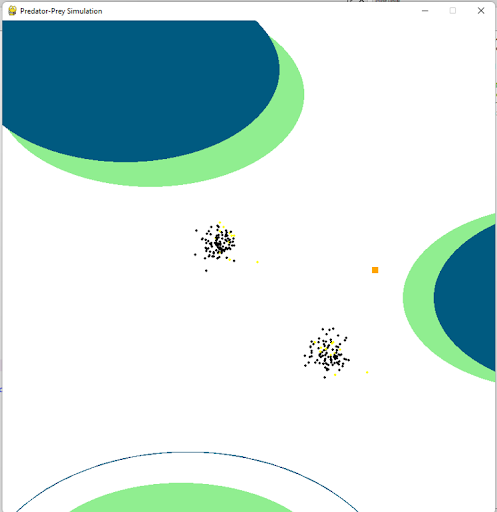
\includegraphics[scale=.5]{figure1.png}%
\captionof{figure}{}\label{labelname}%
\end{center}

\begin{center}
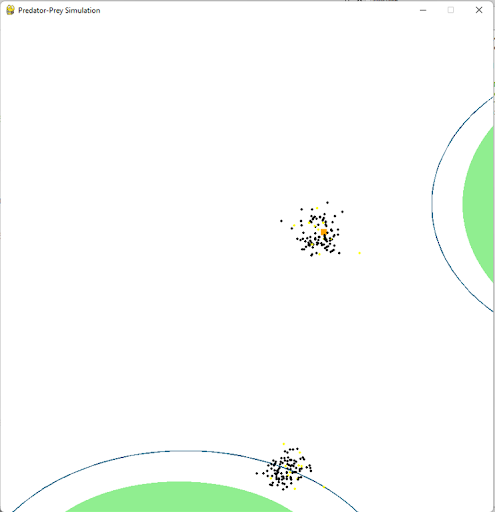
\includegraphics[scale=.5]{figure2.png}%
\captionof{figure}{}\label{labelname}%
\end{center}

Figure 1 depicts two herds of water buffalo partially through their flocking simulation during the wet season. Figure 2 depicts the same as Figure 1 except during the dry season and with the predator engaging one of the buffalo herds (seen by the orange square [the predator] moving through the upper herd). Both of these images were taken at 120 clock cycles/simulation steps and  as you can see from the qualitative data, the bottom herd moved much farther and much quicker during the dry season when compared to the wet season. This is what is expected and helps to validate that our model is performing as expected.

\begin{center}
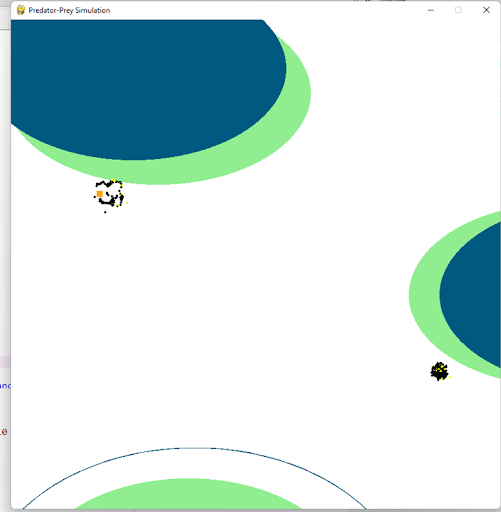
\includegraphics[scale=.5]{figure3.png}%
\captionof{figure}{}\label{labelname}%
\end{center}

Figure 3 depicts a later stage flocking simulation during the wet season where the predator is again breaking up a herd of water buffalo. You can see in Figure 3 that both of the herds are attracted to the resources, but when the predator approaches (seen by the orange square engaging the upper herd), the herd scatters to evade danger. You will also notice in this figure that the herd on the right hand side has yellow dots on the inside of the black dots. These yellow dots are the young water buffalo and they are centered around the older water buffalo (represented by the black dots) creating the ring-like protective structure that we discovered in our research. All of these behaviors are expected in our simulation and reflect our research which again provides validation to our model.


\section*{Quantitative Data}

\begin{center}
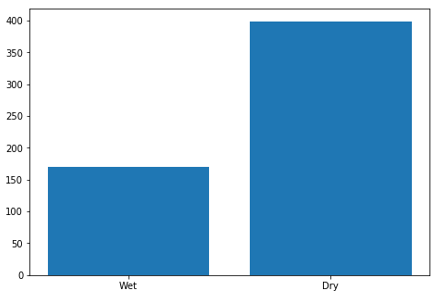
\includegraphics[scale=.5]{figure4.png}%
\captionof{figure}{}\label{labelname}%
\end{center}

\begin{center}
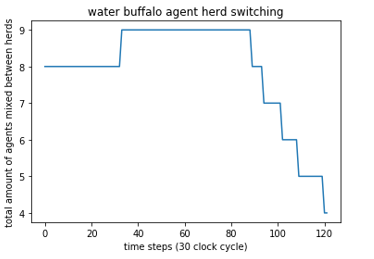
\includegraphics[scale=.6]{figure5.png}%
\captionof{figure}{}\label{labelname}%
\end{center}

\begin{center}
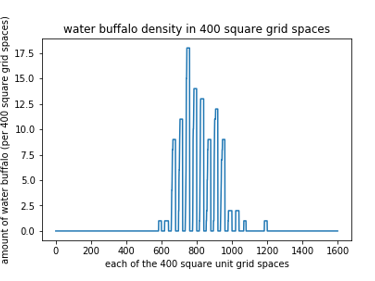
\includegraphics[scale=.6]{figure6.png}%
\captionof{figure}{}\label{labelname}%
\end{center}

\begin{center}
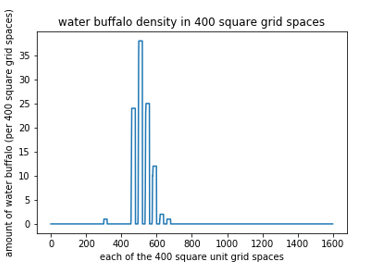
\includegraphics[scale=.6]{figure7.png}%
\captionof{figure}{}\label{labelname}%
\end{center}

Figure 4 is used to further highlight what we observed in Figures 1 and 2, which is the fact that the water buffalo move larger distances in the dry season. As seen in Figure 4, during the dry season, the water buffalo moved more than double the distance (399.19 grid spaces) when compared to the wet season (170.55 grid spaces).

Figure 5 is used to confirm that herd switching was taking place in the model. Over a series of time steps, the total number of agents that had switched herds were being tracked, you can see that early in the simulation/season as the water buffalo are more spread and moving towards their resources, there are more agents switching herds (max calculated was 9 at a given time). You will also see that as the season/simulation progresses, the number of agents switching decreases. This is because the herds become more established and more compact as they begin to flock together and move towards their resources. This behavior was expected in our model and again further validates our simulation.
Figure 6 and 7 are used to show how the density of the water buffalo changes over time with respect to their flocking. Figure 6 is the density calculated at the beginning of the season/simulation (total population/400 square grid spaces). At the beginning of the simulation, the water buffalo are more spread out because they had not fully established their herds yet. This is seen by there being a maximum of about 18 water buffalo per 400 grid spaces. Now if we look at Figure 7, which was captured at the end of the simulation, we can see that there are many more water buffalo per 400 square grid spaces (about a maximum of 40 water buffalo). This is due to the fact that the water buffalo herds are flocking closer together throughout the simulation and becoming more compact. This data reflects our research and provides more validation to our model.

Overall, we have been able to collect sufficient data to validate our model for the features we were trying to capture. When looking at water buffalo movements to find resources, avoid predators, protect their young, and mix herds, our model successfully portrays these systems within our created environment.

\section*{Conclusion}

This report provides a model for water buffalo movement in the wet and dry seasons, with a predator present, when protecting young, all while managing to collect resources. Previous research from tracking data showed that water buffalo move less in the wet season and more in the dry season. Additionally, previous research showed that water buffalo move more in the dry season and find smaller bodies of water and move less in the wet season and find larger bodies of water. Our research also showed how herd switching and protecting young work, which we successfully modeled in our simulation. By creating an accurate model that incorporated multiple elements of water buffalo movement, we were able to show all of these insights to be true. Modeling animal habitat selection is becoming increasingly important, and especially with animals reliant on their environment. Drastic changes in the climate can affect these species directly, and understanding their movement patterns can help us with preservation efforts. Not only will this work help protect water buffaloes, but it will help other species as well.

\section*{Project Contributions}

George Khoury: Created first version of simulation with environment and buffalo herd. Altered flocking code to create realistic movement patterns for the buffalo herd. Created initial draft of paper and converted paper to a journal style with LATEX. I would agree that we both made big contributions to the project. 

Eric Prologo: Worked to implement attractions and repulsions as well as the dynamics of protecting the young water buffalo into the simulation for the herds. Also added additional resources to the environment. Generated graphs for the results of our model. Overall, I felt that we both contributed equally and contributed quality work to our project.

\newpage

\begin{quote}
{\bf References and Notes}

\begin{enumerate}
\item “Buffalo Facts: Southern Africa Wildlife Guide.” {\it Buffalo Facts | Southern Africa Wildlife Guide,} \url{https://www.nathab.com/know-before-you-go/african-safaris/southern-africa/wildlife-guide/buffalo/}
\item Colli, Licia, et al. “New Insights on Water Buffalo Genomic Diversity and Post-Domestication Migration Routes from Medium Density SNP Chip Data.” Frontiers in Genetics, {\it Frontiers in Genetics,} 1 Jan. 1AD, \url{https://www.frontiersin.org/articles/10.3389/fgene.2018.00053/full#:~:text=Based%20on%20a%20geographical%20analysis,swamp%20buffaloes%20migrated%20from%20northern.}
\item Hays, Jeffrey. “Water Buffaloes: Characteristics, Behavior and Wild Ones.” {\it Facts and Details,} \url{https://factsanddetails.com/asian/cat62/sub408/entry-2830.html.}
\item Lewis, Betty. “Bison vs. Oxen.” {\it Pets on Mom.com,} 19 Nov. 2020, \url{https://animals.mom.com/bison-vs-oxen-4883.html.}
\item Roug, A., Muse, E.A., Clifford, D.L. et al. {\it Seasonal movements and habitat use of African buffalo in Ruaha National Park, Tanzania.} BMC Ecol 20, 6 (2020).
\item Tsiobani, E. T., Yiakoulaki, M. D., Hasanagas, N. D., \& Antoniou, I. E. (2020). {\it Proximity patterns in water buffaloes' activities on pasture.} Archives animal breeding, 63(1), 19–29. \url{https://doi.org/10.5194/aab-63-19-2020}
\item Tulloch, DG. “Season Movement and Distribution of the Sexes in the Water Buffalo, Bubalus Bubalis, in the Northern Territory.” {\it Australian Journal of Zoology,} CSIRO PUBLISHING, 1970, \url{https://www.publish.csiro.au/ZO/ZO9700399}
\end{enumerate}
\end{quote}


\end{document}




















